\chapter{\textsc{Tavor CLI}}
\label{chapter:tavorCLI}

The \textsc{Tavor CLI} is the command line interface (CLI) for the \textsc{Tavor framework}. It is therefore the user interface for non-programmers to utilize the capabilities of the framework for fuzzing and delta-debugging. Commands and arguments have to be specified for the binary using the following format:

\begin{center}
\texttt{<general arguments> <command> <command arguments>}
\end{center}

General arguments, which are listed in detail in Listing~\ref{lst:tavor-cli-general-arguments} of Appendix~\ref{chapter:AppendixTavorCLI}, are mostly just activating the output of textual logs for informing the user or to set global constants. Arguments are applied during initialization or the invocation of a CLI command. Examples for global constants are the \texttt{---seed} argument, which sets the seed for the random generator of the CLI to make all executions deterministic, and the \texttt{---max-repeat} argument, which sets the maximum repetition for unrolling loops. The CLI acts on a \textsc{Tavor format} file which is specified by the \texttt{---format-file} argument.

The \textsc{Tavor CLI}'s main purpose is the invocation of the following CLI commands:

\begin{itemize}
\item The \texttt{graph} command converts the given format file into a graphical representation.
\item The \texttt{fuzz} command produces fuzzed outputs from the given format file.
\item The \texttt{validate} command applies the given format file to a specified input file.
\item The \texttt{reduce} command applies delta-debugging for the given format file to a specified input.
\end{itemize}

The following sections describe these commands, their arguments, workflow and usage in more detail.

\nottitlecapsection{\titlecap{Command }\texttt{graph}}
\label{sec:tavor-cli-graph}

The \texttt{graph} command of the \textsc{Tavor CLI} converts a given \textsc{Tavor format} file to a graphical representation of a finite-state machine (FSM). This functionality is needed because textual representations of graphs, such as the \textsc{Tavor format}, are often too difficult to mentally visualize. Listing~\ref{lst:tavor-cli-graph-arguments} of Appendix~\ref{chapter:AppendixTavorCLI} presents the available arguments for this command. Most notable is the \texttt{---filter} argument which allows to define \texttt{fuzzing filters} before the graphical conversion is executed. The command outputs the textual DOT graph description language~\footnote{\url{http://www.graphviz.org/content/dot-language}}, which can be further processed into image formats, e.g., by using the Graphviz toolset~\footnote{\url{http://www.graphviz.org}}.

Figure~\ref{fig:cli-workflow-graph} illustrates the workflow and the interactions of components for the \texttt{graph} command. First the user-specified \textsc{Tavor format} file is read in from the file system and parsed using the format parser of the framework, which results into a \texttt{token graph}. Then optional \texttt{fuzzing filters} are applied to the graph. As last step in the workflow the graph converter component of the framework is used, to convert the \texttt{token graph} to textual DOT formated data for the FSM which is streamed to the STDOUT file descriptor of the CLI.

\begin{figure}[t]
\includegraphics[width=1.0\textwidth]{images/cli-workflow-graph.pdf}
\caption{Workflow for the \texttt{graph} command of the \textsc{Tavor CLI}}
\label{fig:cli-workflow-graph}
\end{figure}

The algorithm for the conversion of the \texttt{token graph} to DOT data is composed by the following two phases:

\begin{listing}[H]
\caption{Convert \texttt{Token Graph} to Simple Graph Structure}
\label{lst:tavor-cli-convert-token-graph}
\begin{gocode}
func buildGraph(token, graph) start, end {
  start, end = {}, {}
  switch type(token) {
    Optional:
      token' = token.Child()
      start', end' = buildGraph(token', graph)

      start.AddOptional(start')
      end.AddOptional(end')
    Concatenation:
      prev = {}
      for i = 0; i < token.NumChildren; i++ {
        token' = token.Child(i)
        start', end' = buildGraph(token', graph)

        graph.AddEdges(prev, start')

        if start'.ContainsOptional() {
          start'.Add(prev)
        }
        prev = start'

        if i == 0 {
          start = start'
        } else if i == token.NumChildren-1 {
          end = end'
        }
      }
    Scope:
      token' = token.Child()
      start' end = buildGraph(token', graph)
    String:
      graph.AddState(token)

      start = {token}
      end = {token}
  }
  return start, end
}
\end{gocode}
\end{listing}

\begin{itemize}
\item Phase one traverses the \emph{token graph} using a recursive depth-first search, which builds upon the assumption, that the used data structure does not contain any loops. As mentioned in Subsection~\ref{subsec:tokens-advanced-concepts}, a loop unrolling step is performed after the format has been parsed to make sure that there are no loops in the token graph. Since each \emph{token type} has its own representation and internal data structure, each type has to be treated differently for the graphical representation using its own implementation. The pseudo code for handling \emph{Optional}, \emph{Concatenation}, \emph{Scope} and \emph{String Tokens} is shown in Listing~\ref{lst:tavor-cli-convert-token-graph}. The traversal function receives the current token to process as well as the graph data structure which needs to be extended. As return values it delivers the set of start and end states of the extended graph data structure.
When traversing an Optional Token, the returned start and end states need to be marked as optional. In case of processing a Concatenation Token, edges need to be added to the graph data structure which connect the individual children of the Concatenation Token. The returned start (resp. end) states are the start (resp. end) states of the first (resp. last) child of the Concatenation Token. When traversing a Scope Token a call to process its only child is performed. Whenever a String Token is processed, a state is added to the resulting graph. As String Tokens are leaves of the token graph no further recursive calls are necessary.
\item Phase two uses the extended graph structure as well as the returned start and end states of phase one to print a DOT representation of the input token graph. End states are depicted using double lines around their label. Optional vertices are shown by using dashed incoming and outgoing arrows. Additional labels and states, which are not included in the pseudo code, are used to depict other tokens such as repeating groups and ranges.
\end{itemize}

The \textsc{Tavor format} in Listing~\ref{lst:tavor-cli-graph-example-tavor} exemplifies how the \texttt{graph} command works. The format results in the DOT data depicted in Listing~\ref{lst:tavor-cli-graph-example-dot} of Appendix~\ref{chapter:AppendixTavorCLI}, which is convertible into the FSM illustrated in Figure~\ref{fig:tavor-cli-graph-example-svg}. All tokens of the format, which are depicted in the graphics as states, are sequential but the tokens $B$ and $F$ are optional, and the group $D E$ is repeated at least twice but at most four times. States are connected using different types of edges, which are depicted as differently styled arrows in the graphics. The FSM depicted in Figure~\ref{fig:tavor-cli-graph-example-svg} starts with the small dot at the top of the graphics. Since $B$ is optional, its incoming and outgoing arrows are dotted. In contrast, the arrow from $A$ to $C$ is solid and is therefore mandatory. However, since $A$ has two outgoing arrows, only one of them has to be taken. Figure~\ref{fig:tavor-cli-graph-example-svg} also illustrates repetition of the $D E$ group, which is indicated by the small dot with an ingoing arrow that has a label with the repetition amount. This arrow causes a loop, therefore marking the repetition. Finally, the accepting state after the repetition has a double bordered circle. Each path of a graph must end in such an accepting state, or else it is not a valid path, i.e., it is not considered by the fuzzing and delta-debugging processes. In this example, it is also possible to go from the accepting state after the repetition to the $F$ token which is optional but also ends in an accepting state.

\begin{figure}[t]
\centering
\begin{minipage}{.5\textwidth}
  \centering
  \begin{listing}[H]
  \caption{Example \textsc{Tavor format} for the \texttt{graph} command}
  \label{lst:tavor-cli-graph-example-tavor}
  \begin{gocode}
  START = A ?(B) C +2,4(D E) ?(F)

  A = "a"
  B = "b"
  C = "c"
  D = "d"
  E = "e"
  F = "f"
  \end{gocode}
  \end{listing}
\end{minipage}%
\begin{minipage}{.5\textwidth}
  \centering
  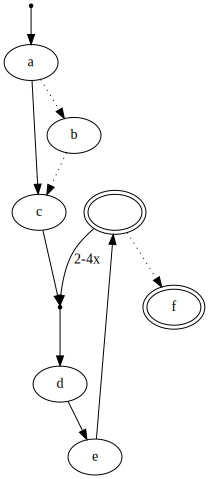
\includegraphics[width=0.5\textwidth]{images/tavor-cli-graph-example.pdf}
  \captionof{figure}{Example graphics for the \texttt{graph} command}
  \label{fig:tavor-cli-graph-example-svg}
\end{minipage}
\end{figure}

\nottitlecapsection{\titlecap{Command }\texttt{fuzz}}
\label{sec:tavor-cli-fuzz}

The \texttt{fuzz} command of the \textsc{Tavor CLI} generates permutations, which conform to a specified format. Additionally, it is capable of forwarding these permutations to external programs, thus allowing to systematically execute a system under test with a stream of inputs for some predefined structure.

Figure~\ref{fig:cli-workflow-fuzz} illustrates the workflow and the interactions of components for the \texttt{fuzz} command. It starts along the same lines as the \texttt{graph} command, by first parsing the \textsc{Tavor format} file into a \texttt{token graph} and by applying optional \texttt{fuzzing filters} on that graph. It then proceeds with its fuzzing loop, which uses a specified \texttt{fuzzing strategy} to generate consecutive permutations. These permutations are written either to the file system or the STDOUT file descriptor. External programs may process these permutations and in turn interact with the \textsc{Tavor CLI} using their exit codes or via STDIN.

\begin{figure}[t]
\hspace*{-1cm}\includegraphics[width=1.1\textwidth]{images/cli-workflow-fuzz.pdf}
\caption{Workflow for the \texttt{fuzz} command of the \textsc{Tavor CLI}}
\label{fig:cli-workflow-fuzz}
\end{figure}

The fuzzing loop of the \texttt{fuzz} command is highly configurable via command line options, which are listed in Listing~\ref{lst:tavor-cli-fuzz-options} of Appendix~\ref{chapter:AppendixTavorCLI}. It may either interact with executables or scripts. When working with executables their exit codes as well as their STDOUT and STDERR file descriptors are processed by the fuzzing loop. In case the \texttt{---exit-on-error} option is set the fuzzing loop will terminate in case an unexpected output is encountered in any of the afore mentioned communication channels. When using scripts the communication with the fuzzing loop is solely performed via STDIN and STDOUT. The fuzzing loop writes permutations separated by a predefined separator to STDIN of the script and waits until the script signals via its STDOUT that it has processed the current permutation. Success or failure, are signaled by using the constants \enquote{Yes} and \enquote{No}.

\begin{figure}[b]
\hspace*{-1cm}\begin{tabular}{cc}
\subfloat[Direct fuzzing of a program]{\includegraphics[scale=0.53]{images/cli-fuzz-simple-validation.pdf}\label{fig:cli-fuzz-external-programs-simple}}
\hspace*{0.3cm}\subfloat[Usage of an interposed validation executable]{\includegraphics[scale=0.53]{images/cli-fuzz-exec-validator.pdf}\label{fig:cli-fuzz-external-programs-val}}
\end{tabular}
\caption{Fuzzing of external programs}\label{fig:cli-fuzz-external-programs}
\end{figure}

When using the \textsc{Tavor CLI} to immediately fuzz an external program there are two ways to proceed, which are depicted in Figure~\ref{fig:cli-fuzz-external-programs}. Either the program under test is directly passed on to the \textsc{Tavor CLI}, or an interposed validation executable is used. To communicate directly with the program under test has the advantage that only the expected input format is required to start fuzzing. But also has the downside that the built-in validating capabilities of the \textsc{Tavor CLI} are restricted to specifying return codes as well as regular expressions on delivered outputs in STDOUT and STDERR. In case a more thorough validation is required, which cannot be accomplished by the afore mentioned validation capabilities, we advise to use interposed executables or scripts. Consider for instance a program which sorts CSV files by specific columns. An interposed validation function or script could not only check that the program under test exits without errors, but could additionally verify that the output CSV is indeed sorted and its content corresponds to the input CSV file. Several examples of customized scripts and executables are provided at~\footnote{\url{https://github.com/zimmski/tavor/tree/master/examples/fuzzing}}.

\nottitlecapsection{\titlecap{Command }\texttt{validate}}
\label{sec:tavor-cli-validate}

The \texttt{validate} command of the \textsc{Tavor CLI} checks that a given input file conforms to a specified format file. This functionality can be helpful since for instance the \texttt{reduce} command only applies delta-debugging on valid inputs, or in the general case it can be used to examine an input, which was not generated through the given format file.

Figure~\ref{fig:cli-workflow-validate} illustrates the workflow and the interactions of components for the \texttt{validate} command. It starts off by parsing the specified \textsc{Tavor format} file to its corresponding token graph. In the next step this token graph is used to parse the specified input file. In case the input file can be parsed successfully, it conforms to the specified format file. The CLI exits with the exit status $0$ if the input file conforms to the format file, or exits with an exit status unequal to $0$ if it does not conform.

Please refer to Listing~\ref{lst:tavor-cli-validate-options} of Appendix~\ref{chapter:AppendixTavorCLI} for a list of available arguments of the \texttt{validate} command.

\begin{figure}[hb]
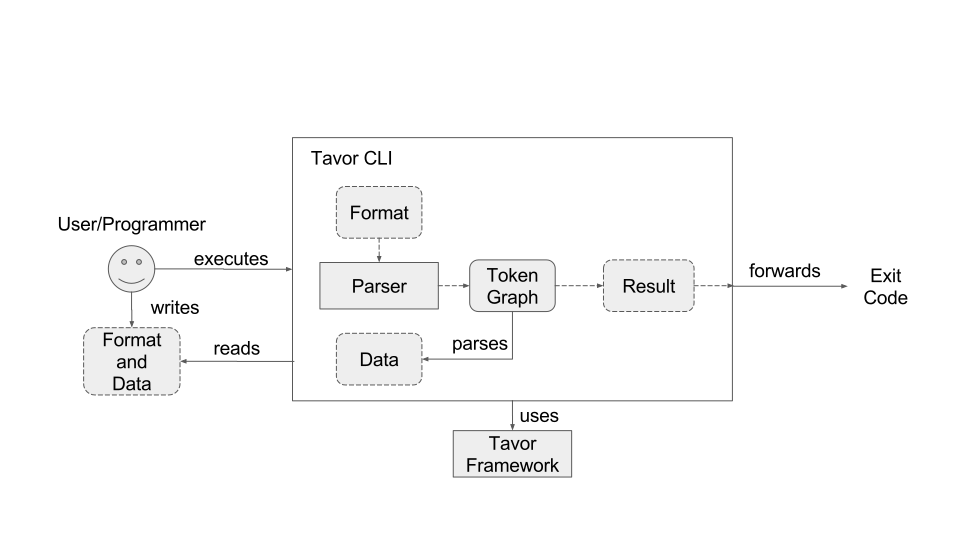
\includegraphics[width=1.0\textwidth]{images/cli-workflow-validate.pdf}
\caption{Workflow for the \texttt{validate} command of the \textsc{Tavor CLI}}
\label{fig:cli-workflow-validate}
\end{figure}


\nottitlecapsection{\titlecap{Command }\texttt{reduce}}
\label{sec:tavor-cli-reduce}

The \texttt{reduce} command applies delta-debugging to a given input according to a specified \textsc{Tavor format} file, i.e., given an input which results in certain program behavior, this capability may be used to systematically reduce the given input while preserving the same behavior.

Figure~\ref{fig:cli-workflow-reduce} depicts the workflow and the interactions of components for the \texttt{reduce} command. It starts similar to the \texttt{validate} command by first parsing the \textsc{Tavor format} file to its associated token graph. This graph is then used to parse the given input data, i.e., the initial input needs to correspond to the specified format. Next, the reduction loop starts by feeding the initial input data to an external resource and capturing its responses. These initial responses are consecutively used by the reduction loop to guide the generation of reduced inputs, i.e., only reductions resulting in these responses are investigated for further reductions.

\begin{figure}[hb]
\includegraphics[width=1\textwidth]{images/cli-workflow-reduce.pdf}
\caption{Workflow for the \texttt{reduce} command of the \textsc{Tavor CLI}}
\label{fig:cli-workflow-reduce}
\end{figure}

Various options are available for the \texttt{reduce} command, which are listed in Listing~\ref{lst:tavor-cli-reduce-options} of Appendix~\ref{chapter:AppendixTavorCLI}. The \texttt{reduce} command works along the same lines as the \texttt{fuzz} command, i.e., it may interact with scripts or executables using exit codes as well as STDERR, STDOUT and STDIN as communication channels. Options such as \texttt{---exec-match-stderr} allow to define the expected structure of outputs written to those channels. Please refer to~\footnote{\url{https://github.com/zimmski/tavor/tree/master/examples/deltadebugging}} for example scripts and executables for performing delta-debugging.

\begin{listing}[H]
\caption{Delta-debugging pseudo code for scripts}
\label{lst:tavor-cli-delta-debug-scripts}
\begin{gocode}
func deltaDebugScript(tokenGraph, reduceStrategy) {
  continue, feedback = reduceStrategy(tokenGraph)

  for i = range continue {
    stdin.Write(tokenGraph.String())
    stdin.Write(inputSeparator)

    result = stdout.ReadLine()
    switch result {
      case "YES\n":
        feedback <- Good
      case "NO\n":
        feedback <- Bad
    }

    continue <- i
  }
}
\end{gocode}
\end{listing}

Consider Listing~\ref{lst:tavor-cli-delta-debug-scripts}, which outlines the pseudo code of the reduction loop when working with scripts. A token graph, which holds the parsed input data, as well as the reducing strategy, for reducing the input data, are passed on to function~\texttt{deltaDebugScript}. The reducing strategy receives in Line~2 the token graph to operate on, and returns two channels. In order to communicate that the current processing step is finished the channel \texttt{continue} is used, i.e., the call in Line~4 blocks until the reducing strategy has produced another permutation. The channel \texttt{feedback} is used to signal whether the current permutation still triggers the expected behavior, thus steering the reducing strategy.
